\documentclass[10pt]{beamer}

\mode<presentation>{% Settings
    % link to view http://www.hartwork.org/beamer-theme-matrix/
    % ------------------------------------------------------------------------------
    % Slide Themes
    % ------------------------------------------------------------------------------
    %\usetheme{default}
    %\usetheme{AnnArbor}
    %\usetheme{Antibes}
    %\usetheme{Bergen}
    \usetheme{Berkeley}
    %\usetheme{Berlin}
    %\usetheme{Boadilla}
    %\usetheme{CambridgeUS}
    %\usetheme{Copenhagen}
    %\usetheme{Darmstadt}
    %\usetheme{Dresden}
    %\usetheme{Frankfurt}
    %\usetheme{Goettingen}
    %\usetheme{Hannover}
    %\usetheme{Ilmenau}
    %\usetheme{JuanLesPins} % rounded title, gradient at top with section, no bottom bar
    %\usetheme{Luebeck}     % square title, toc at top of each slide
    %\usetheme{Madrid}      % rounded title
    %\usetheme{Malmoe}
    %\usetheme{Marburg}
    %\usetheme{Montpellier}
    %\usetheme{PaloAlto}
    %\usetheme{Pittsburgh}
    %\usetheme{Rochester}
    %\usetheme{Singapore}
    %\usetheme{Szeged}
    %\usetheme{Warsaw}

    % ------------------------------------------------------------------------------
    % Color Schemes
    % ------------------------------------------------------------------------------
    %\usecolortheme{default}
    %\usecolortheme{albatross}  % blue background with darker blue
    %\usecolortheme{beaver}     % gray with red
    %\usecolortheme{beetle}     % gray background
    %\usecolortheme{crane}      % orange
    \usecolortheme{dolphin}     % white with purple
    %\usecolortheme{dove}       % all white
    %\usecolortheme{fly}        % all gray including background
    %\usecolortheme{lily}       % white with blue
    %\usecolortheme{orchid}     % default blue
    %\usecolortheme{rose}       % default blue
    %\usecolortheme{seagull}    % darker gray than seahorse
    %\usecolortheme{seahorse}   % light gray blueish tint
    %\usecolortheme{whale}      % default blue
    %\usecolortheme{wolverine}  % yellow with a little blue

    %\setbeamertemplate{footline} % To remove the footer line in all slides uncomment this line
    %\setbeamertemplate{footline}[page number] % To replace the footer line in all slides with a simple slide count uncomment this line
    \setbeamertemplate{navigation symbols}{} % To remove the navigation symbols from the bottom of all slides uncomment this line
    \setbeamertemplate{bibliography item}{\insertbiblabel} % to number bibliography entries
}

\usepackage{Logemann}
\usepackage{Integral}
\usepackage{LinearAlgebra}
\usepackage{Derivative}
\usepackage{Vector}
\usepackage{Sum}
\usepackage{SetTheory}
\usepackage[backend=biber]{biblatex}
\addbibresource{refs.bib}

\title[]{Discontinuous Galerkin Method for Solving Thin Film Equations} % The short title
% appears at the bottom of every slide, the full title is only on the title page

\author{Caleb Logemann} % Your name
\institute[Iowa State University]{% Your institution as it will appear on the bottom of every slide, may be shorthand to save space
Mathematics Department, Iowa State University \\ % Your institution for the title page
\medskip
\textit{logemann@iastate.edu}} % Your email address

\date{December 13, 2018} % Date, can be changed to a custom date

\begin{document}
  \begin{frame}
    \titlepage{}
  \end{frame}

  \begin{frame}
    \frametitle{Overview}
    \tableofcontents
  \end{frame}

  \section{Introduction}
    \begin{frame}
      \frametitle{Motivation}
      \begin{itemize}
        \item Aircraft Icing
        \item Runback
      \end{itemize}
      \begin{center}
        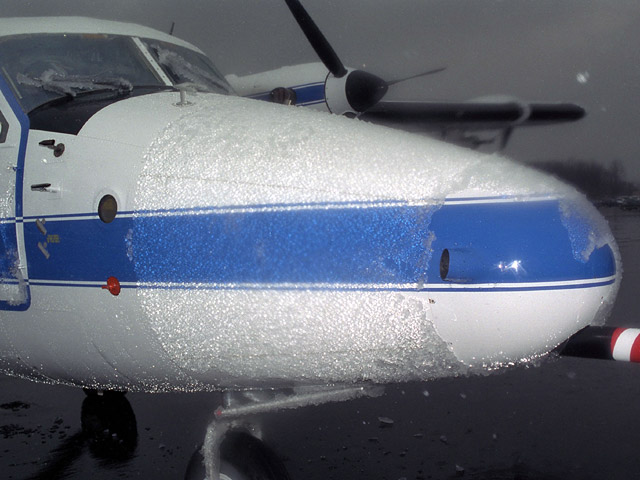
\includegraphics[scale=0.2]{Figures/Icing_on_a_plane.jpg}
        \hspace{0.1in}
        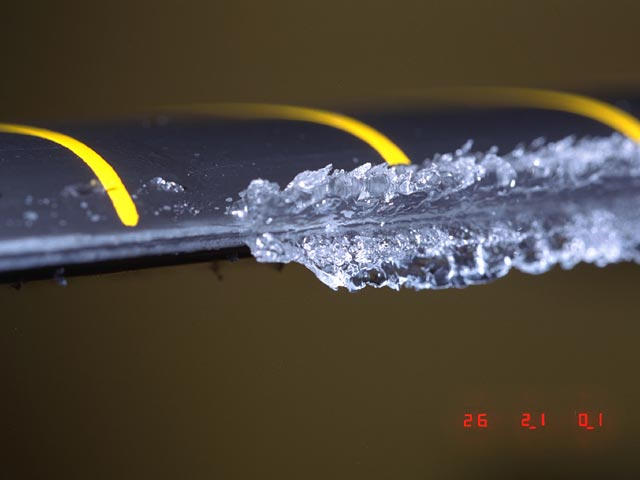
\includegraphics[scale=0.2]{Figures/Icing_on_a_rotor.jpg}
      \end{center}
      \begin{itemize}
        \item Industrial Coating
      \end{itemize}
    \end{frame}

    \begin{frame}
      \frametitle{Model Equations}
      \begin{itemize}
        \item Navier-Stokes Equation
          \begin{align*}
            \nabla \cdot \v{u} &= 0 \\
            \partial_t \v{u} + \nabla \cdot \p{\v{u}\v{u}} &= - \frac{1}{\rho} \nabla p + \frac{1}{\rho}\nabla \cdot \sigma + \v{g} \\
            \partial_t h_s + \p{u, v}^T \cdot \nabla h_s &= w \\
            \partial_t h_b + \p{u, v}^T \cdot \nabla h_b &= w
          \end{align*}
        \item Lubrication or reduced Reynolds number approximation
        \item Thin-Film Equation - 1D with $q$ as fluid height.
          \[
            q_t + \p{f(x, t) q^2 - g(x, t) q^3}_x = -\p{h(x, t) q^3 q_{xxx}}_x
          \]
      \end{itemize}
    \end{frame}

  \section{Method}
    \begin{frame}
      \frametitle{Operator Splitting}
      \begin{itemize}
        \item Simplified Model
          \[
            q_t + \p{q^2 - q^3}_x = -\p{q^3 q_{xxx}}_x \qquad \p{0, T} \times \Omega
          \]

        \item Operator Splitting
          \begin{align*}
            q_t + \p{q^2 - q^3}_x &= 0 \\
            q_t + \p{q^3 u_{xxx}}_x &= 0
          \end{align*}

        \item Strang Splitting \hfill \\
          $\frac{1}{2}\Delta t$ step of Convection
          \[
            q_t + \p{q^2 - q^3}_x = 0
          \]
          $\Delta t$ step of Diffusion
          \[
            q_t + \p{q^3 u_{xxx}}_x = 0
          \]
          $\frac{1}{2}\Delta t$ step of Convection
          \[
            q_t + \p{q^2 - q^3}_x = 0
          \]
      \end{itemize}
    \end{frame}

  \subsection{Convection}
    \begin{frame}
      \frametitle{Convection}
      \begin{itemize}
        \item Convection Equation
          \begin{gather*}
            q_t + f\p{q}_x = 0 \qquad \p{0, T} \times \Omega \\
            f(q) = q^2 - q^3
          \end{gather*}

        \item Weak Form \hfill \\
          Find $q$ such that
          \[
            \dintt*{\Omega}{}{q_t v - f(q) v_x}{x} = 0
          \]
          for all test functions $v$
      \end{itemize}
    \end{frame}

    \begin{frame}
      \frametitle{Notation}
      \begin{itemize}
        \item Partition the domain, $\br{a, b}$ as
          \[
            a = x_{1/2} < \cdots < x_{j-1/2} < x_{j+1/2} < \cdots < x_{N + 1/2} = b
          \]

        \item $I_j = \br{x_{j-1/2}, x_{j+1/2}}$
        \item $x_j = \frac{x_{j+1/2} + x_{j-1/2}}{2}$.
          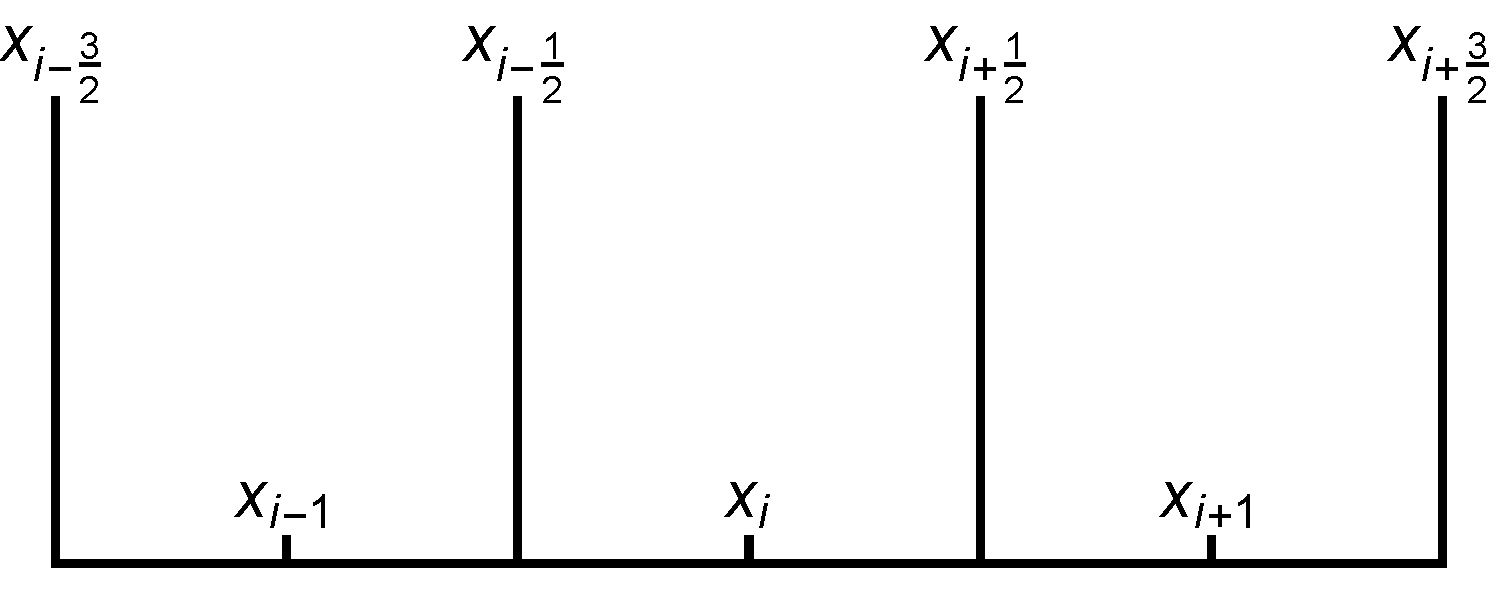
\includegraphics[scale=0.35]{Figures/Cells.pdf}
      \end{itemize}
    \end{frame}

    \begin{frame}
      \frametitle{Runge Kutta Discontinuous Galerkin}
      \begin{itemize}
        \item 
          Find $Q(t,x)$ such that for each time $t \in \p{0, T}$, $Q(t, \cdot) \in V_h = \set{v \in L^1(\Omega): \eval{v}{I_j} \in P^k(I_j)}$
          \begin{align*}
            \dintt{I_j}{}{Q_t v}{x} &= \dintt{I_j}{}{f(Q)v_x}{x} \\
            &- \p{\mcF_{j + 1/2}v^-(x_{j+1/2}) - \mcF_{j - 1/2}v^+(x_{j-1/2})}
          \end{align*}
          for all $v \in V_h$

        \item Rusanov/Local Lax-Friedrichs Numerical Flux
          \small{
          \[
            \mcF_{j+1/2} = \frac{1}{2}\p{f\p{Q^-_{j+1/2}} + f\p{Q^+_{j+1/2}}} + \max[q]{\abs{f'(q)}}\p{Q^-_{j+1/2} - Q^+_{j+1/2}}
          \]}
        \vspace{-.3cm}
        \item Solve this system of ODEs with any Explicit Strong Stability Preserving (SSP) Runge-Kutta Method.
      \end{itemize}
    \end{frame}

    \begin{frame}
      \frametitle{Explicit SSP Runge Kutta Methods}
      \begin{itemize}
        \item Forward Euler
          \begin{align*}
            q^{n+1} = q^n + \Delta t L(q^n)
          \end{align*}

        \item Second Order
          \begin{align*}
            q^{\star} &= q^n + \Delta t L(q^n) \\
            q^{n+1} &= \frac{1}{2}\p{q^n + q^{\star}} + \frac{1}{2} \Delta t L(q^{\star})
          \end{align*}
      \end{itemize}
    \end{frame}

  \subsection{Diffusion}
    \begin{frame}
      \frametitle{Diffusion}
      \begin{itemize}
        \item Diffusion Equation
          \begin{align*}
            q_t &= -\p{q^3 q_{xxx}}_x \qquad \p{0, T} \times \Omega
          \end{align*}

        \item Linearize operator at $t = t^n$, let $f(x) = q^3(t = t^n, x)$
          \[
            q_t = -\p{f(x) q_{xxx}}_x \qquad \p{0, T} \times \Omega
          \]
      \end{itemize}
    \end{frame}

    \begin{frame}
      \frametitle{Finite Difference Approach}
      \begin{itemize}
        \item Let cell centers, $x_i$ form finite difference grid.
        \item Finite difference space, $\RR^N$.
        \item $Q_{DG} \in V_h \to Q_{FD} \in \RR^N$
          \[
            \p{Q_{FD}}_i = \frac{1}{h}\dintt{K_i}{}{Q_{DG}}{x}
          \]

        \item $Q_{FD} \in \RR^N \to Q_{DG} \in V_h$
          \begin{align*}
            \eval{Q_{DG}}{K} &\in P^1(K) \\
            \frac{1}{h}\dintt{K_i}{}{Q_{DG}}{x} &= \p{Q_{FD}}_i \\
            \eval{\partial_x Q_{DG}}{K_i} &= \frac{\p{Q_{FD}}_{i+1} - \p{Q_{FD}}_{i-1}}{2h}
          \end{align*}
      \end{itemize}
    \end{frame}

    \begin{frame}
      \frametitle{Finite Difference Approximation}
      \begin{align*}
        \p{q_{xxx}}_{i+1/2} &\approx \frac{-Q_{i-1} + 3Q_i - 3Q_{i+1} + Q_{i+2}}{h^3} \\
        F_{i+1/2} &= \frac{f(x^+_{i+1/2}) + f(x^-_{i+1/2})}{2} \\
        \p{-\p{f(x) q_{xxx}}_x}_i &\approx -\frac{F_{i+1/2}\p{q_{xxx}}_{i+1/2} - F_{i-1/2}\p{q_{xxx}}_{i-1/2}}{h}
      \end{align*}
    \end{frame}

    %\begin{frame}
      %\frametitle{Local Discontinuous Galerkin}
      %Find $Q(t, x), R(x), S(x), U(x)$ such that for all $t \in \p{0, T}$
      %$Q(t, \cdot), R, S, U \in V_h = \set{v \in L^1(\Omega): \eval{v}{I_j} \in P^k(I_j)}$
      %\begin{align*}
        %\eta &= Q^3 \\
        %\dintt{I_j}{}{R v}{x} &= -\dintt{I_j}{}{Q v_x}{x} + \p{\hat{Q}_{j+1/2}v^-_{j+1/2} - \hat{Q}_{j-1/2} v^+_{j-1/2}} \\
        %\dintt{I_j}{}{S w}{x} &= -\dintt{I_j}{}{R w_x}{x} + \p{\hat{R}_{j+1/2}w^-_{j+1/2} - \hat{R}_{j-1/2} w^+_{j-1/2}} \\
        %\dintt{I_j}{}{U y}{x} &= \dintt{I_j}{}{S_x \eta y}{x} - \p{S^-_{j+1/2}\eta^-_{j+1/2}y^-_{j+1/2} - S^+_{j-1/2}\eta^+_{j-1/2}y^+_{j-1/2}} \\
        %&+ \p{\hat{S}_{j+1/2} \hat{\eta}_{j+1/2} y^-_{j+1/2} - \hat{S}_{j-1/2} \hat{\eta}_{j-1/2} y^+_{j-1/2}} \\
        %\dintt{I_j}{}{Q_t z}{x} &= -\dintt{I_j}{}{U z_x}{x} + \p{\hat{U}_{j+1/2}z^-_{j+1/2} - \hat{U}_{j-1/2} z^+_{j-1/2}}
      %\end{align*}
      %for all $I_j \in \Omega$ and all $v, w, y, z \in V_h$.
    %\end{frame}

    %\begin{frame}
      %\frametitle{Numerical Fluxes}
      %\begin{align*}
        %\hat{\eta}_{j+1/2} &= \frac{1}{2}\p{\eta^+_{j+1/2} + \eta^-_{j+1/2}} \\
        %\hat{Q}_{j+1/2} &= Q^+_{j+1/2} \\
        %\hat{R}_{j+1/2} &= R^-_{j+1/2} \\
        %\hat{S}_{j+1/2} &= S^+_{j+1/2} \\
        %\hat{U}_{j+1/2} &= U^-_{j+1/2}
      %\end{align*}
      %\begin{center}
        %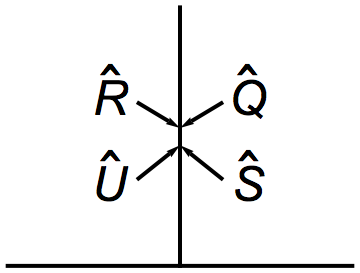
\includegraphics[scale=0.3]{Figures/localDG.png}
      %\end{center}
    %\end{frame}

    \begin{frame}
      \frametitle{Implicit L-Stable Runge Kutta}
      \begin{itemize}
        \item Backward Euler
          \begin{align*}
            q^{n+1} = q^n + \Delta t L(q^{n+1})
          \end{align*}

        \item 2nd Order
          \begin{align*}
            q^{\star} &= q^n + \frac{1}{4} \Delta t \p{L(q^n) + L(q^{\star})} \\
            3 q^{n+1} &= 4 q^{\star} - q^{n} + \Delta t L(q^{n+1})
          \end{align*}
      \end{itemize}
    \end{frame}

    %\begin{frame}
      %\frametitle{Linear Solver}
      %\begin{itemize}
        %\item Generalized Minimal Residual (GMRES)
          %\begin{gather*}
            %\min[x \in K_n]{\norm{A\v{x} - \v{b}}} \\
            %K_n = \spanspace{\v{b}, A\v{b}, A^2\v{b}, \ldots, A^{n-1}\v{b}} 
          %\end{gather*}

        %\item Preconditioned
          %\begin{align*}
            %P &= A^{-1}_0 \\
            %PAx &= Pb
          %\end{align*}
      %\end{itemize}
    %\end{frame}

  \section{Numerical Results}
    \begin{frame}
      \frametitle{Riemann Problem}
      \begin{center}
        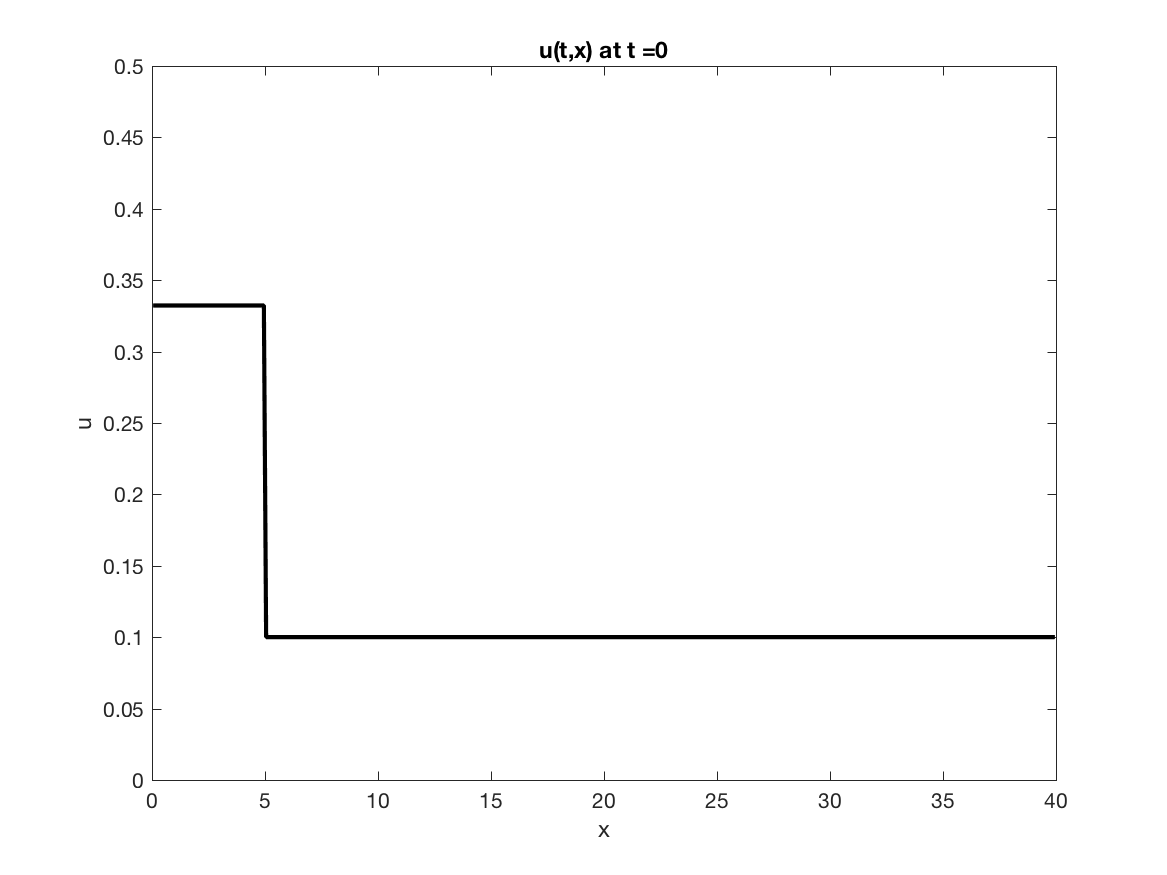
\includegraphics[scale=0.5]{Figures/reimann0.png}
      \end{center}
    \end{frame}
    %\begin{frame}
      %\frametitle{Numerical Results - Riemann Problem}
      %\begin{center}
        %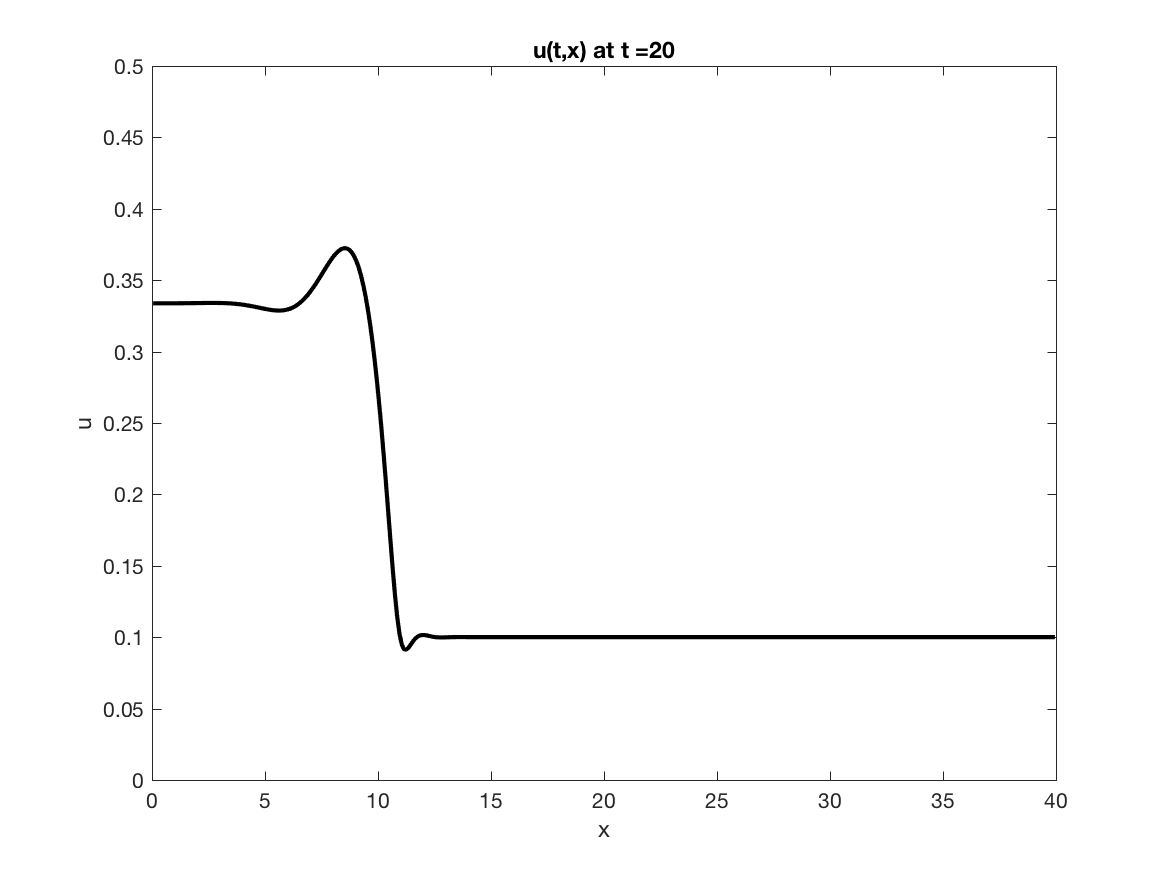
\includegraphics[scale=0.5]{Figures/reimann20.png}
      %\end{center}
    %\end{frame}
    %\begin{frame}
      %\frametitle{Numerical Results - Riemann Problem}
      %\begin{center}
        %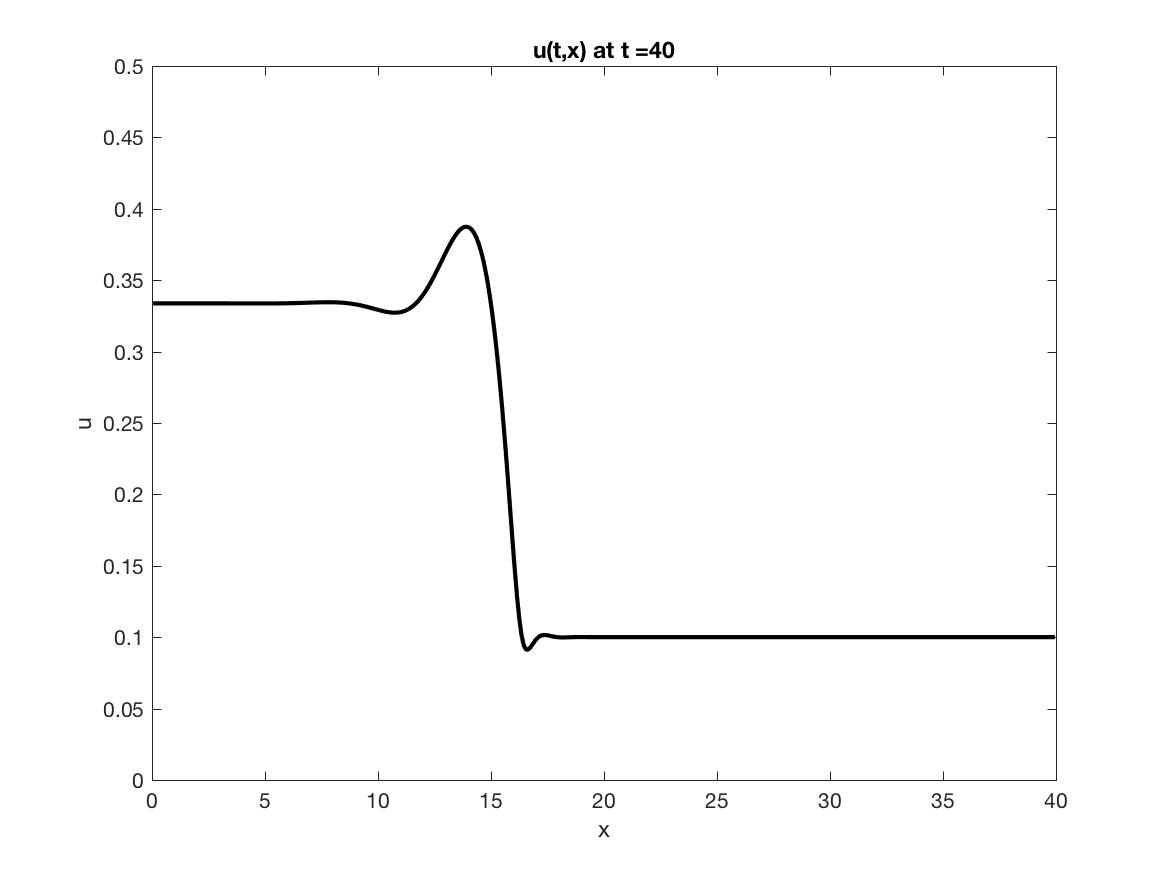
\includegraphics[scale=0.5]{Figures/reimann40.png}
      %\end{center}
    %\end{frame}
    \begin{frame}
      \frametitle{Riemann Problem}
      \begin{center}
        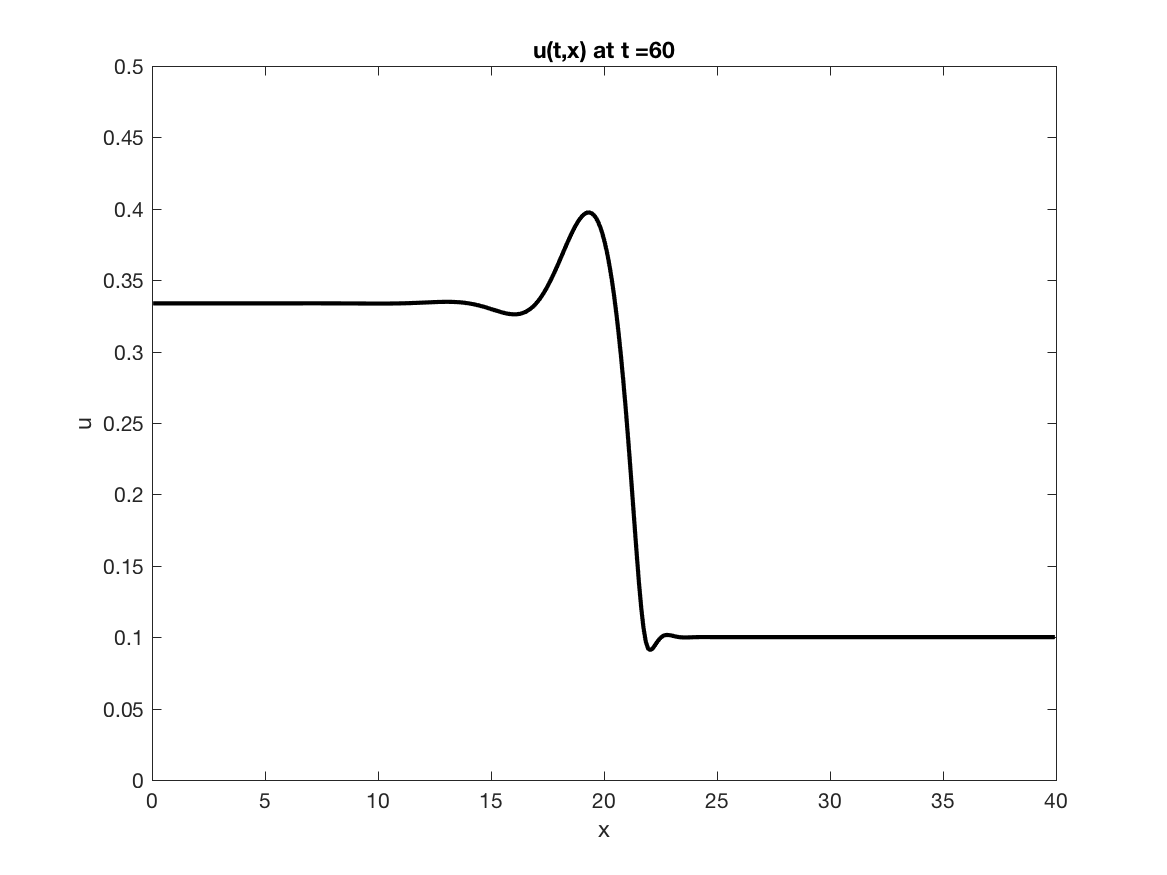
\includegraphics[scale=0.5]{Figures/reimann60.png}
      \end{center}
    \end{frame}
    %\begin{frame}
      %\frametitle{Numerical Results - Riemann Problem}
      %\begin{center}
        %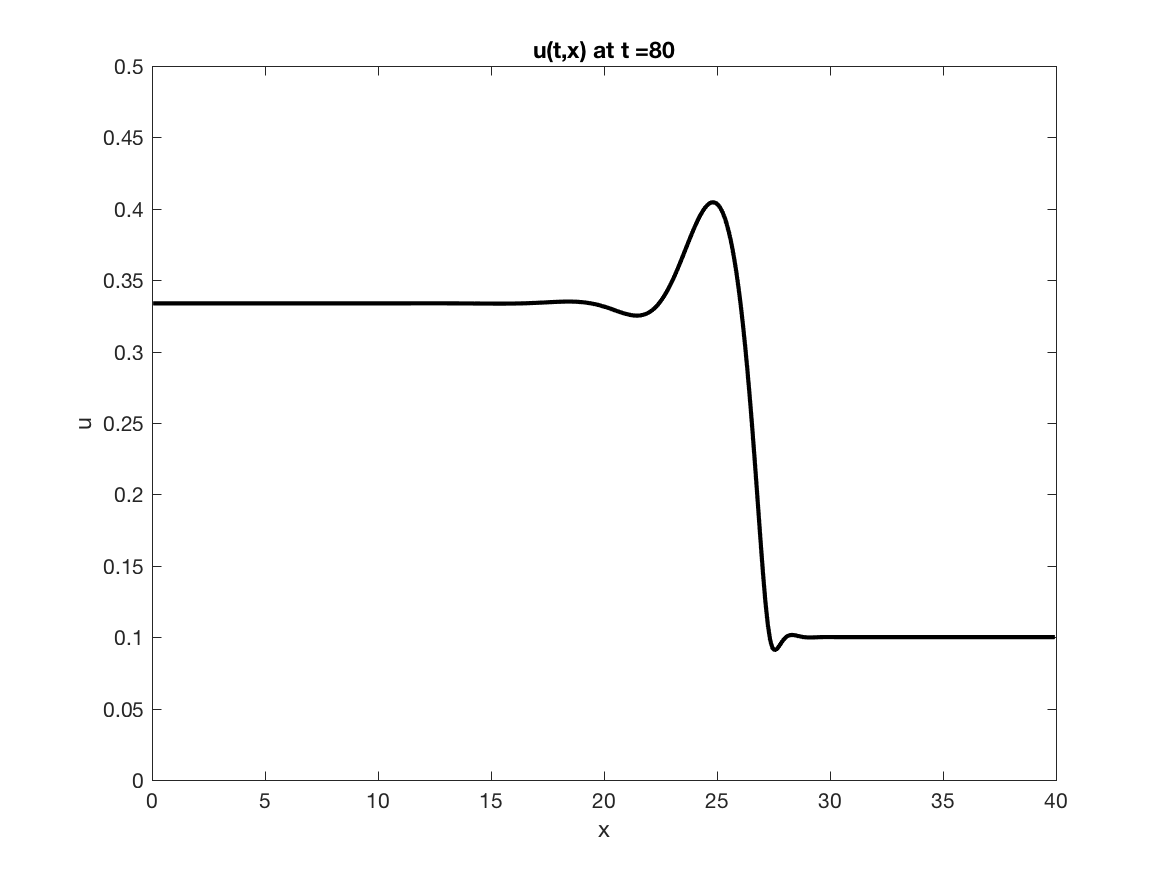
\includegraphics[scale=0.5]{Figures/reimann80.png}
      %\end{center}
    %\end{frame}
    %\begin{frame}
      %\frametitle{Numerical Results - Riemann Problem}
      %\begin{center}
        %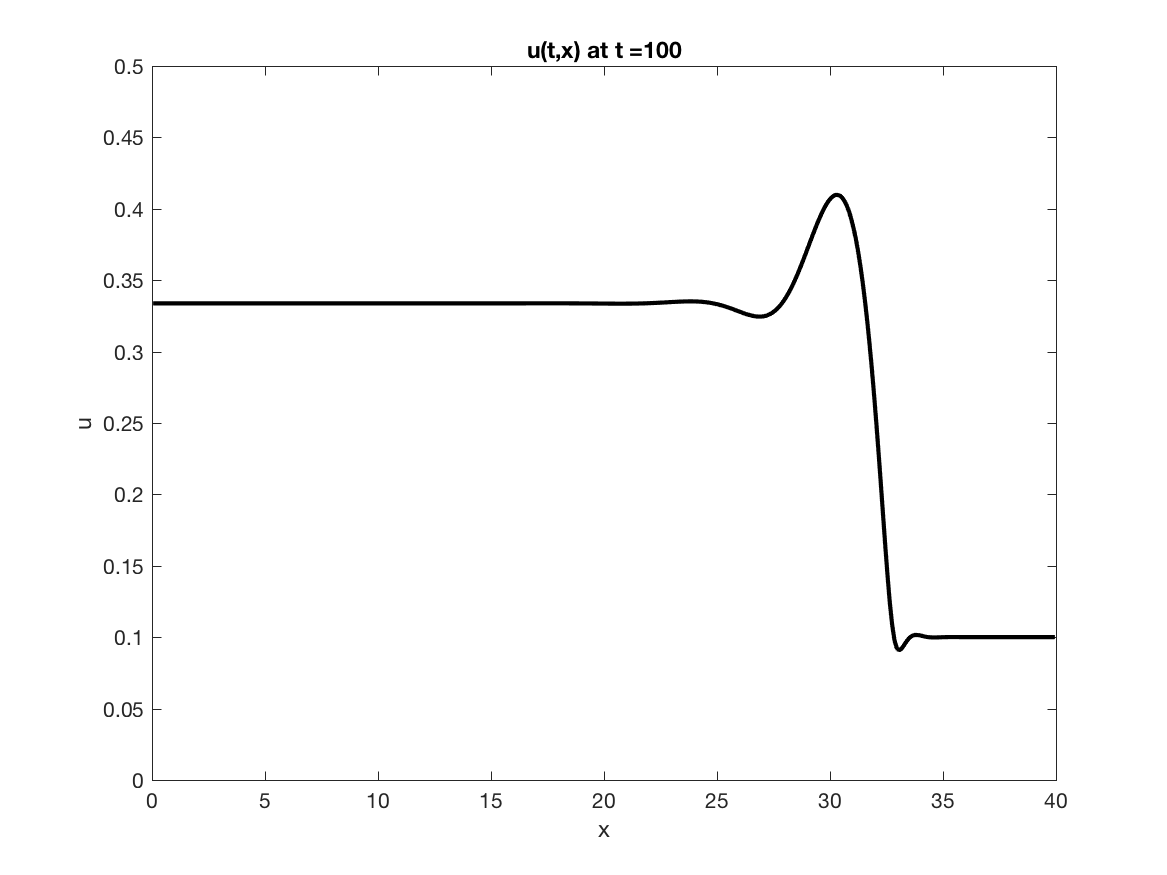
\includegraphics[scale=0.5]{Figures/reimann100.png}
      %\end{center}
    %\end{frame}

    \begin{frame}
      \frametitle{Square Wave}
      \begin{center}
        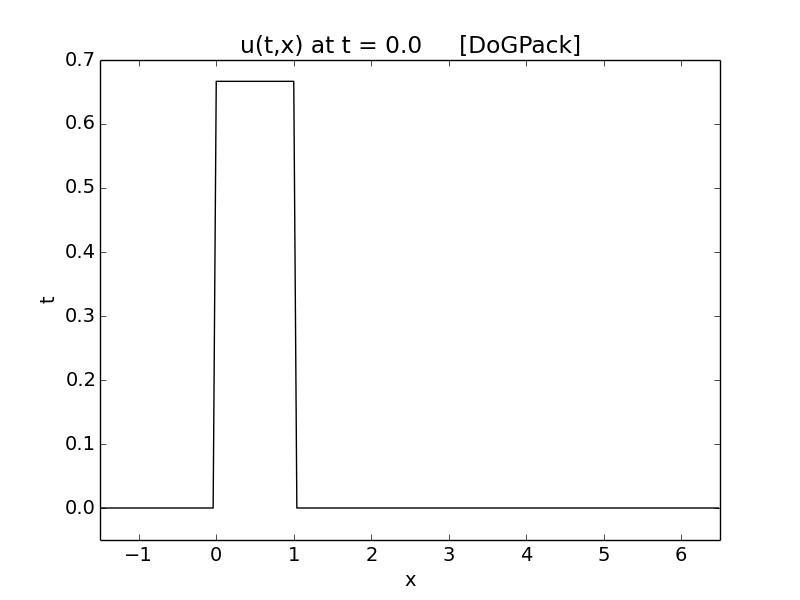
\includegraphics[scale=0.5]{Figures/squareWaveInitial.png}
      \end{center}
    \end{frame}
    \begin{frame}
      \frametitle{Square Wave}
      \begin{center}
        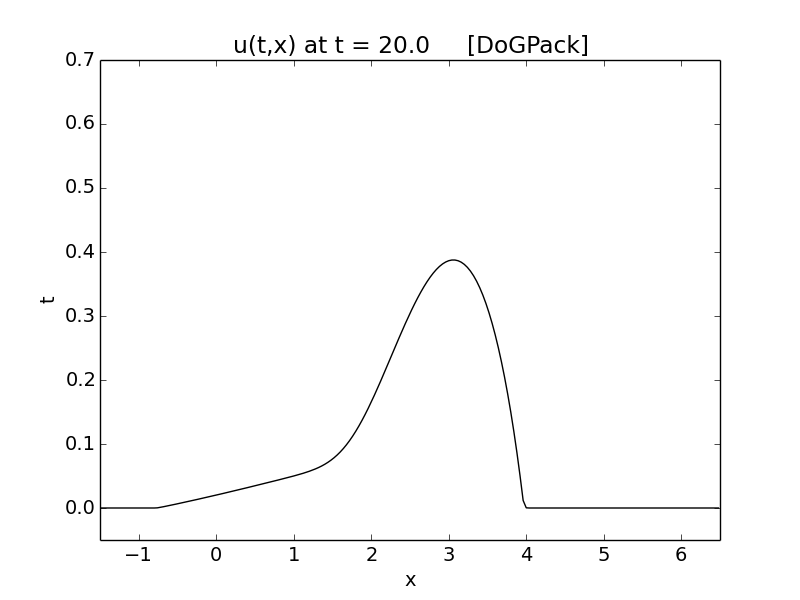
\includegraphics[scale=0.5]{Figures/squareWaveFinal.png}
      \end{center}
    \end{frame}

  \section{Conclusion}
    \begin{frame}
      \frametitle{Future Work}
      \begin{itemize}
        \item Show second order convergence
        \item Runge Kutta IMEX
        \item Space and time dependent coefficients
      \end{itemize}
    \end{frame}

    \begin{frame}
      \frametitle{Bibliography}
      % TODO: Bibliography
      \nocite{*}
      \printbibliography{}
    \end{frame}
\end{document}
